\section{Estado del Arte}

% qué métodos se han usado para resolverlo?
% cuáles son los mejores algoritmos que se han creado hasta la fecha?
% qué representaciones han tenido los mejores resultados?
% cuál es la tendencia actual para resolver el problema?
% tipos de movimientos
% heurísticas
% métodos completos
% tendencias
% incluye gráficos comparativos o explicativos

% No hay justificación para esta decisión, la sección del estado del arte es la más importante en esta entrega y la que amerita mayor discusión y opinión propia del alumno.

% No se discute acerca de las representaciones usadas en los experimentos.

% No se expresan conclusiones respecto al por qué de los resultados mostrados. Se debe explicar por qué ciertas técnicas funcionan mejor que otras y bajo qué formulaciones del problema.

% No se discute acerca de tendencias de nuevas investigaciones

% Solo se toma en cuenta un resultado de un experimento y no se analizan las técnicas por separado.


En esta sección del trabajo no se discutirán los detalles de los algoritmos estudiados, porque no es parte esencial de este trabajo, solamente se dispondrá información recopilada sobre las diferentes técnicas utilizadas en la literatura para resolver de la forma más óptima este problema combinacional.
Los algoritmos estudiados serán Tabu Search, Simulated Annealing, Genetic Algorithm y Variable Neighborhood Search.

% Figuras mal organizadas
En al figura \ref{fig_comparison} se muestra una comparación realizada en un estudio del problema de los algoritmos antes mencionados, dispuestos como TS, SA, GA y VNS, este gráfico nos muestra el tiempo en unidades de CPU de estos algoritmos a medida que aumentan las iteraciones o escenarios, con un máximo de 19 escenarios.

Se puede notar que los valores de tiempo de CPU se aproximan hasta el escenario 10, después, hay pendientes pronunciadas para GA, TS y especialmente para VNS.
EL tiempo de solución de SA tiene una pendiente muy baja y se puede ver fácilmente que SA supera a estos algoritmos cuando la dimensión del problema es mayor.


\begin{figure}[!ht]
    \centering
    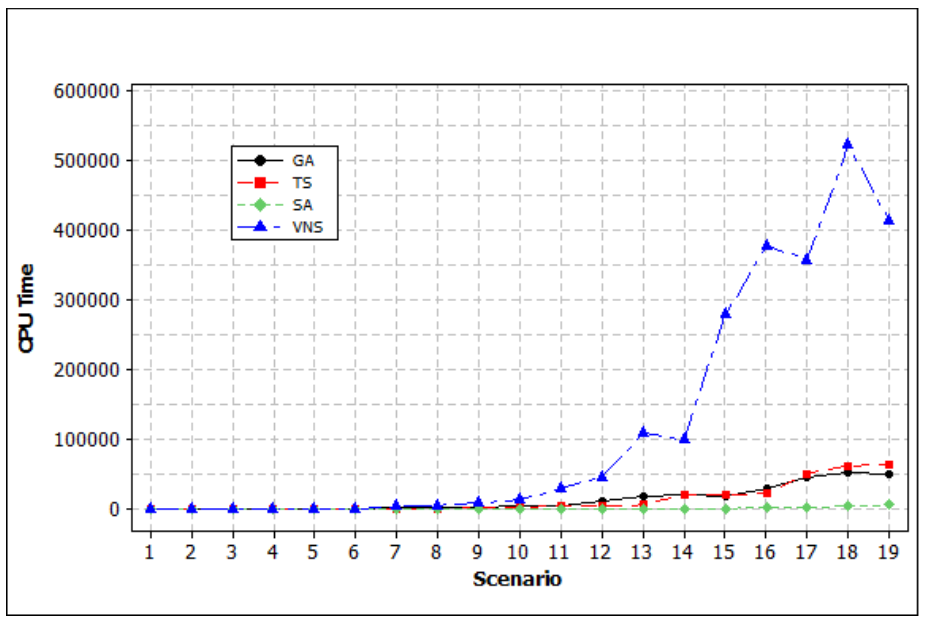
\includegraphics[width=0.8\textwidth]{images/cpu_time_comparasion_of_algorithms.png}
    \caption{CPU Time Comparison of Algorithms \cite[pág 47]{WithTechniques}}
    \label{fig_comparison}
\end{figure}

% \subsection{Genetic Algorithm}
% \subsection{Tabu Search}
% \subsection{Simulated Annealing}
% \subsection{Variable Neighborhood}
